%% Los capitulos inician con \chapter{T'itulo}, estos aparecen numerados y
%% se incluyen en el 'indice general.
%%
%% Recuerda que aqu'i ya puedes escribir acentos como: 'a, 'e, 'i, etc.
%% La letra n con tilde es: 'n.

\chapter{Desarrollo e Implementación}

En este capítulo se explican en detalle los procesos que fueron necesarios para implementar el sistema tomando en cuenta la arquitectura planteada en el capitulo anterior. 

\section{Implementación de Módulos}

	A continuación se aprecia la implementación de cada uno de los módulos que componen el sistema para inferir la deserción de los clientes en un e-commerce.
	
\subsection{Modelo}

El objetivo de este módulo es generar un modelo en el formato PKL, para esto se decidió crear un programa utilizando la tecnología Jupyter Notebook. El proceso se realizó en fases:

\subsubsection{Instalación de dependencias}

La primera fase consiste en importar las dependencias necesarias para realizar el análisis, preprocesamiento y generar el modelo:

\begin{lstlisting}[language=Python, caption=Importar dependencias en modelo.ipynb]
import pandas as pd
import datetime
from lifetimes import BetaGeoFitter
from lifetimes.plotting import plot_frequency_recency_matrix
from lifetimes.plotting import plot_probability_alive_matrix
from lifetimes.plotting import plot_period_transactions
from lifetimes.plotting import plot_calibration_purchases_vs_holdout_purchases
from lifetimes.plotting import plot_history_alive
from lifetimes.utils import summary_data_from_transaction_data
from lifetimes.utils import calibration_and_holdout_data
\end{lstlisting}

\subsubsection{Cargar el Dataset}

El Dataset que se va a utilizar contiene los datos de transacciones de ventas de una tienda de comercio electrónico con sede en el Reino Unido. Esta tienda de Londres vende regalos y artículos para el hogar y sus clientes provienen de todo el mundo.

El conjunto de datos contiene 500.000 Filas y 8 columnas en las cuales esta representadas las transacciones de ventas de la tienda durante un año. Las columnas son las siguientes:

\begin{itemize}
	\item \textbf{TransactionNo (categórico):} un número único de seis dígitos que define cada transacción. La letra “C” en el código indica una cancelación.
	\item \textbf{Date (numérico):} la fecha en que se generó cada transacción.
	\item \textbf{ProductNo (categórico):} un carácter único de cinco o seis dígitos que se utiliza para identificar un producto específico.
	\item \textbf{Product (categórico):} nombre del producto/artículo.
	\item \textbf{Price (numérico):} el precio de cada producto por unidad en libras esterlinas (£).
	\item \textbf{Quantity (numérico):} la cantidad de cada producto por transacción. Valores negativos relacionados con transacciones canceladas.
	\item \textbf{CustomerNo (categórico):}  un número único de cinco dígitos que define a cada cliente.
	\item \textbf{Country (categórico):} nombre del país donde reside el cliente.
\end{itemize}

Hay un pequeño porcentaje de cancelación de pedidos en el conjunto de datos. La mayoría de estas cancelaciones se debieron a condiciones de falta de existencias en algunos productos. En esta situación, los clientes tienden a cancelar un pedido porque quieren que todos los productos se entreguen de una vez. Los datos se cargan desde el archivo CSV utilizando la biblioteca Pandas.

\begin{lstlisting}[language=Python, caption=Cargar Dataset en modelo.ipynb]
transactional_data = pd.read_csv('../data/Sales Transaction v.4a.csv')
\end{lstlisting}

\subsubsection{Preprocesamiento de los Datos}

Para poder trabajar correctamente con los datos, es necesario que estos cumplan con los formatos esperados de la biblioteca lifetimes y que los datos sean válidos, para ello se realizaron las siguientes operaciones sobre el dataset:

\begin{enumerate}
	\item Se removió la información de precio, país, producto y cantidad ya que no es necesaria para el análisis.
	\item Las transacciones canceladas se van a considerar en el modelo como una interacción de parte del cliente, por lo tanto no se eliminarán.
	\item Varios productos pueden pertenecer a una misma transacción, para representar esto, el dataset contiene entradas con el mismo número de transacción pero con productos diferentes, como solo es necesario saber si se realizó una transacción y no importan los detalles de la misma, se eliminarán las entradas duplicadas.
	\item Es necesario transformar los datos en el campo de fecha al formato datetime de Python.
\end{enumerate}

El código que realiza este preprocesamiento es el siguiente:

\begin{lstlisting}[language=Python, caption=Preprocesamiento en modelo.ipynb]
# Operacion 1
transactional_data = transactional_data.drop(columns=['Price', 'Quantity', 'Country', 'ProductName', 'ProductNo'])

# Operacion 3
transactional_data = transactional_data.drop_duplicates(subset=['TransactionNo'])

# Operacion 4
transactional_data['Date'] = pd.to_datetime(transactional_data['Date'], format='%m/%d/%Y')
\end{lstlisting}

\subsubsection{Formato de datos RFM}

Los modelos BTYD y especificamente la biblioteca lifetimes reciben como entrada datos en formato RFM, esto quiere decir que debemos llevar los datos transaccionales a una tabla RFM.

Para transformar nuestra data transaccional a data RFM utilizamos la función summary\_data\_from\_transaction\_data de la biblioteca lifetimes.
	
\begin{lstlisting}[language=Python, caption=Formato RFM en modelo.ipynb]
rfm_data = summary_data_from_transaction_data(transactional_data, 'CustomerNo', 'Date', observation_period_end='2019-12-31')
\end{lstlisting}

\subsubsection{Ajustar el modelo}

Finalmente se va crear un modelo BG/NBD con la data RFM que representa el comportamiento de los clientes del dataset, para ello se utiliza la clase BetaGeoFitter de la biblioteca lifetimes.

\begin{lstlisting}[language=Python, caption=Ajustar Modelo en modelo.ipynb]
model = BetaGeoFitter()
model.fit(rfm_data['frequency'], rfm_data['recency'], rfm_data['T'])
\end{lstlisting}

\subsubsection{Guardar modelo}

La clase BetaGeoFitter de lifetimes posee una rutina que permite guardar el modelo en un formato PKL para poder ser usado posteriormente.

\begin{lstlisting}[language=Python, caption=Guardar Modelo en modelo.ipynb]
model.save_model('../api/modelo.pkl')
\end{lstlisting}

\subsection{API}

Para implementar la API en el lenguaje de programación Python, se utilizó la biblioteca Flask que abstrae toda la funcionalidad relacionada con programar un servidor web. Esta biblioteca se encarga de implementar todas las reglas del protocolo HTTP.

	El objetivo de la API es crear una ruta HTTP que exponga el recurso conditional-probability-alive, el cual permite calcular la probabilidad de vida de uno o mas clientes. El código del servidor web es el siguiente:
	
\begin{lstlisting}[language=Python, caption=main.py]
# Dependencias
import datetime
import pandas as pd
from flask import Flask, request
from flask_cors import CORS
from lifetimes import BetaGeoFitter
from lifetimes.utils import summary_data_from_transaction_data
from lifetimes.utils import calculate_alive_path

# Cargar Modelo
model = BetaGeoFitter()
model.load_model("./modelo.pkl")

app = Flask(__name__)
CORS(app)

# Ruta para verificar la salud del servidor
@app.route("/")
def index():
    return "Index Page"

# Recurso
@app.route("/conditional-probability-alive", methods=["POST"])
def conditionalProbabilityAlive():
    if request.method == "POST":
        customer_field = "customer"
        date_field = "date"
        data = request.json["transactions"]

        # Validaciones
        if data.get("customer") is None or data.get("date") is None:
            return "Bad Request", 400

        if type(data.get("customer")) not in (tuple, list):
            return "Bad Request", 400

        if type(data.get("date")) not in (tuple, list):
            return "Bad Request", 400

        if len(data.get("date")) != len(data.get("customer")):
            return "Bad Request", 400

        df = pd.DataFrame.from_dict(data)
        rfm_data = summary_data_from_transaction_data(df, customer_field, date_field)
        rfm_data["p_alive"] = model.conditional_probability_alive(
            rfm_data["frequency"], rfm_data["recency"], rfm_data["T"]
        )
        result = rfm_data.to_dict("index")

        for i, _row in rfm_data.iterrows():
            path = (
                calculate_alive_path(
                    model, df[df[customer_field] == i], date_field, 500
                )
                .to_numpy()
                .tolist()
            )
            result[i]["path"] = [item for sublist in path for item in sublist]
        return {"result": result}
    else:
        raise RuntimeError("Unsupported method {}".format(request.method))
\end{lstlisting}	

Al inicio, el programa importa las dependencias necesarias para su ejecución: Pandas, datetime, lifetimes y Flask; luego de esto, se inicializa y carga el modelo, acto seguido, se implementa una ruta de inicio para verificar que el servidor se está ejecutando y finalmente se implementa el recurso objetivo.

	El recurso /conditional-probability-alive recibe una lista de transacciones de clientes, transforma esa información en una tabla RFM que es utilizada como entrada al modelo para calcular el “camino de vida” o probabilidad de que cada cliente esté activo durante 500 días luego de la primera transacción.

	El valor de 500 días se puede parametrizar, pero se decidió mantenerlo constante para evitar una sobrecarga del servidor en caso de que se solicite procesar mucha información. Finalmente el recurso retorna toda la información que ha calculado, incluyendo la tabla RFM.
	
\subsection{Aplicación Web}

Para construir la interfaz web se usó Typescript como lenguaje de programación, Vue.js como framework y Nuxt como metaframework para ahorrar tiempo de desarrollo. Vue.js se encarga de abstraer y gestionar todo el dinamismo, mientras que Nuxt provee de una estructura al proyecto y abstrae toda la lógica de compilación, optimización y manejo de dependencias del proyecto. La aplicación esta compuesta de una sola vista llamada “index” donde se representan todos los aspectos de la interfaz. La vista ejecuta varias funciones según la acción del usuario. 

En la programación de la vista se utilizaron variables de estado internas para almacenar la información ingresada por el usuario, realizar cálculos intermedios y guardar la respuesta de la API, estas variables tienen la siguiente definición:

\begin{lstlisting}[language=C++, caption=script en index.vue]
const runtimeConfig = useRuntimeConfig()
const transactions = ref({
  customer: [] as string[],
  date: [] as string[]
})
const newTransaction = ref({
  date: '',
  customer: ''
})
const formErrors = ref({
  date: false,
  client: false
})
const customerData = ref({} as {
   [k: string]: {
      startDate: string,
      transactions: string[]
   }
})
const result = ref({} as {
   [k: string]: {
      p_alive: number,
      dates: string[],
      path: number[]
      T: number,
      recency: number,
      frequency: number
   }
})
\end{lstlisting}	

Cuando el usuario presiona el botón "Registrar" se ejecuta la función "addTransaction", la cual se encarga de validar y registrar una transacción, su implementación es la siguiente:

\begin{lstlisting}[language=C++, caption=addTransaction en index.vue]
function addTransaction () {
  formErrors.value.date = false
  formErrors.value.client = false

  const utc = moment(newTransaction.value.date, 'DD-MM-YYYY', true)

  if (!utc.isValid()) {
    formErrors.value.date = true
  }

  if (!newTransaction.value.customer) {
    formErrors.value.client = true
  }

  if (formErrors.value.date || formErrors.value.client) {
    return false
  }

  transactions.value.customer.push(newTransaction.value.customer)
  transactions.value.date.push(moment(newTransaction.value.date, 'DD-MM-YYYY').format('DD-MM-YYYY'))

  if (!customerData.value[newTransaction.value.customer]) {
    customerData.value[newTransaction.value.customer] = {
      startDate: moment().format('DD-MM-YYYY'),
      transactions: []
    }
  }

  if (moment(customerData.value[newTransaction.value.customer].startDate, 'DD-MM-YYYY') > moment(newTransaction.value.date, 'DD-MM-YYYY')) {
    customerData.value[newTransaction.value.customer].startDate = moment(newTransaction.value.date, 'DD-MM-YYYY').format('DD-MM-YYYY')
  }

  customerData.value[newTransaction.value.customer].transactions.push(moment(newTransaction.value.date, 'DD-MM-YYYY').format('DD-MM-YYYY'))

  newTransaction.value = {
    date: '',
    customer: ''
  }
}
\end{lstlisting}	

Luego de agregar una transacción, se genera una tabla en la interfaz donde se puede ver la información registrada. En cada entrada de la tabla existe un botón para eliminar la transacción que al ser accionado por el usuario ejecuta la función "removeTransaction" que tiene la siguiente implementación:

\begin{lstlisting}[language=C++, caption=removeTransaction en index.vue]
function removeTransaction (id: number) {
  if (id === 0) {
    transactions.value.customer.shift()
    transactions.value.date.shift()
  } else {
    transactions.value.customer.splice(id, 1)
    transactions.value.date.splice(id, 1)
  }
}
\end{lstlisting}	

Luego de que el usuario registre las transacciones que desee, acciona el botón "Predecir" el cual ejecuta la función "predict" y tiene la siguiente lógica:

\begin{lstlisting}[language=C++, caption=predict en index.vue]
async function predict () {
  const response = await $fetch(`${runtimeConfig.public.apiBase}/conditional-probability-alive`, {
    headers: {
      'Content-Type': 'application/json'
    },
    method: 'POST',
    body: {
      transactions: {
        customer: transactions.value.customer,
        date: transactions.value.date.map(e => moment(e, 'DD-MM-YYYY').format('MM/DD/YYYY'))
      }
    }
  }) as any
  result.value = response.result

  for (const customer in result.value) {
    const startDate = customerData.value[customer].startDate
    result.value[customer].dates = generateDates(startDate, 500)
    result.value[customer].path = result.value[customer].path.map(v => Math.floor((1 - v) * 1000) / 10)
  }
}
\end{lstlisting}	

Existe una función auxiliar que genera las fechas diarias desde la menor fecha en una transacción, hasta 500 días luego, su implementación es la siguiente:

\begin{lstlisting}[language=C++, caption=generateDates en index.vue]
function generateDates (start: string, end: number) {
  const dateArray = []
  const currentDate = moment(start, 'DD-MM-YYYY').toDate()
  const endDate = new Date(currentDate)
  	.setDate(currentDate.getDate() + end)

  while (currentDate <= new Date(endDate)) {
    dateArray.push(moment(currentDate).format('DD-MM-YYYY'))
    // Se utiliza UTC date para prevenir problemas con zonas horarios y DST
    currentDate.setUTCDate(currentDate.getUTCDate() + 1)
  }
  return dateArray
}
\end{lstlisting}	

El resultado se muestra en gráficos generados mediante la biblioteca Chart.js, para ello se ejecuta el siguiente código en Vue:

\begin{lstlisting}[language=HTML, caption=crear gráfico en index.vue]
   <div 
   	v-if="Object.keys(result).length"
   	class="m-auto max-w-5xl"
   >
      <h2 class="font-bold text-xl pb-6">
        Resultados
      </h2>
      <div 
      	v-for="(value, name) in result" 
      	:key="name" class="pb-4"
      >
        <h3 class="font-bold">
          Usuario: {{ name }}
        </h3>
        <LineChart
          class="w-full"
          :chart-data="{
            labels: value.dates,
            datasets: [
              {
                data: value.path,
                label: '% Probabilidad de haber desertado',
                spanGaps: true,
                pointRadius: 0,
                borderColor: 'rgba(200, 0, 0, 0.8)',
                backgroundColor: 'rgba(200, 0, 0, 0.2)',
              }
            ]
          }"
          :options="{
            scales: {
              y: {
                ticks: {
                  callback(value: number) {
                    return value + ' %';
                  }
                }
              }
            }
          }"
        />
      </div>
    </div>
\end{lstlisting}	

Finalmente, obtenemos una interfaz completa que cumple con los requerimientos del capitulo anterior y se puede ver en la figura a continuación.

\begin{figure}[H]
	\centering 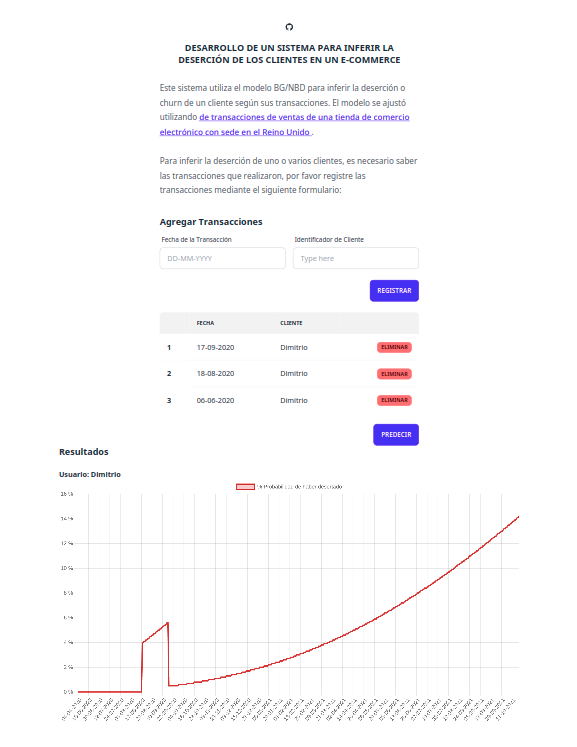
\includegraphics[width=0.90\textwidth]{images/2.png}
	\caption{Vista Index}
	\label{fig:ui_end}
\end{figure}

